\documentclass{deliverablereport}

\deliverable{UI}{ipython-kernels}
\deliverydate{01/02/2018}
\duedate{31/08/2017 (M24)}
\author{Jeroen Demeyer, Sebastian Gutsche, Nicolas M.~Thiéry}

\begin{document}
\maketitle
\tableofcontents

%%%%%%%%%%%%%%%%%%%%%%%%%%%%%%%%%%%%%%%%%%%%%%%%%%%%%%%%%%%%%%%%%%%%%%%%

\section{Introduction}

The \href{https://jupyter.org}{Jupyter Notebook} is a web application
that enables the creation and sharing of executable documents
containing live code, equations, visualizations and explanatory text.
Thanks to a modular design, Jupyter can be used with any computational
system that provides a so-called
\href{https://jupyter.readthedocs.io/en/latest/projects/kernels.html}{\emph{Jupyter kernel}}
to communicate with the notebook.

The Jupyter ecosystem is very large and active:
it is being used as a front-end for scientific research
on a daily basis by many researchers around the world,
and also for teaching (see Section~\ref{teaching}).
The technology goes beyond the notebook interface:
it can also be used for live documentation for example.
There is also JupyterLab, a next-generation web application
allowing users to work even more efficiently.

\ODK therefore promotes Jupyter as user interface of choice:
it is particularly suitable for building modular web based Virtual Research Environments.

This deliverable is a follow-up to \delivref{UI}{ipython-kernels-basic},
which dealt with a first basic version of the Jupyter kernels.
We have improved Jupyter kernels for GAP, PARI/GP, SageMath and Singular.
This means that \ODK's main computational components
now all have a full featured Jupyter kernel.
Additionally, we have also cooperated on the development of the C++ kernel xeus-cling.

All the kernels that we worked on now support syntax highlighting, TAB-completion,
interactive help and graphics. Some of them also support interactive widgets.

%%%%%%%%%%%%%%%%%%%%%%%%%%%%%%%%%%%%%%%%%%%%%%%%%%%%%%%%%%%%%%%%%%%%%%%%

\section{Impact}

The implementation of Jupyter kernels for many computational systems
provides their users with an easy-to-use, modern and uniform user interface.

For the various systems mentioned in this report,
the new Jupyter interface is a lot more user friendly than the traditional
command-line interface.
It also makes it easy for the users to organize and share their work.

Furthermore, implementing Jupyter kernels enabled outsourcing the development of user interfaces
which traditionally had been a time sink for those systems.
For example, SageMath is dropping the development of its old notebook SageNB,
and is instead refocussing its energy on other features.

\subsection{Teaching}\label{teaching}

\begin{figure}\label{AIMS}
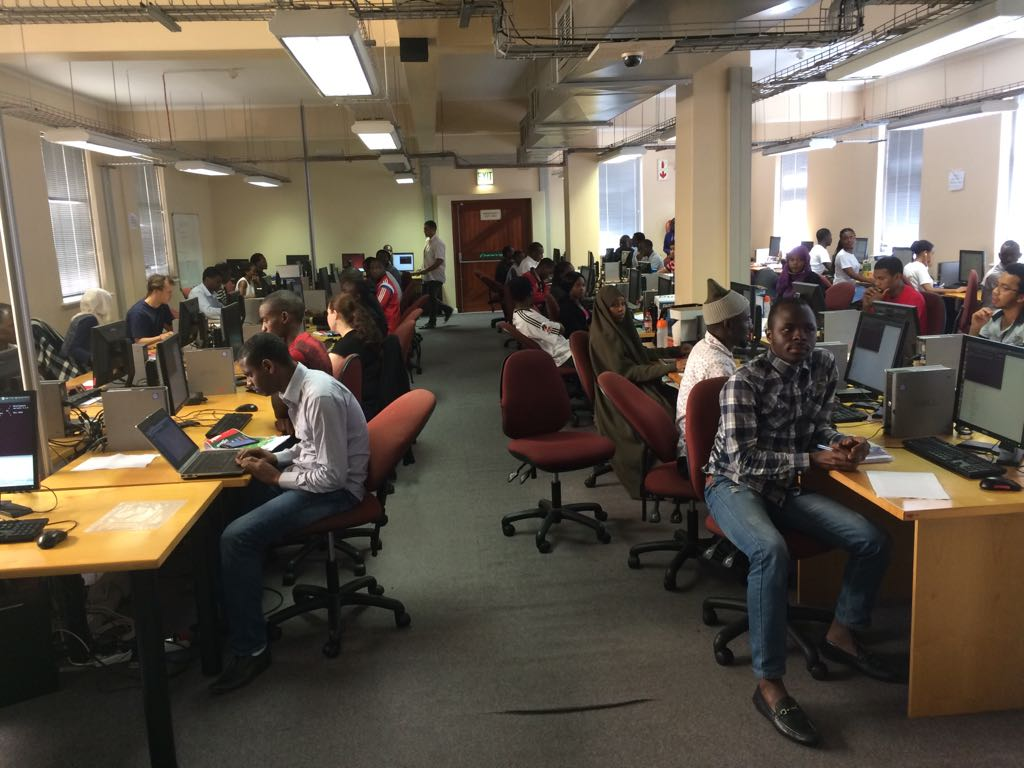
\includegraphics[width=100mm]{IMG-20180124-WA0000.jpg}
\caption{Students at AIMS using the Singular Jupyter interface}
\end{figure}

\begin{itemize}
\item Since 2017, Jupyter is used at Université Paris Sud for teaching C++ to over 300 students.
This was initiated in particular by \ODK participants Loïc Gouarin, Viviane Pons, and Nicolas M.\ Thiéry.
The mix of narrative documents and interactive programming fostered active participation from the students
while our web-based deployment made it easier for them to work from home.
The course material is available from \url{http://Nicolas.Thiery.name/Enseignement/Info111}.

\item In early spring 2017, Prof.~Dr.~W.~Decker and Prof.~Dr.~G.~Pfister gave a
three-week course on computational algebraic geometry at the
African Institute for Mathematical sciences (Cape Town, South Africa)
with lectures and computer lab sessions.
The course was attended by about 50 students from all over Africa.
In the lab sessions, the students learned how to experiment with the computer algebra system Singular.
It proved extremely valuable that the students could run Singular in the Jupyter notebook.

\item The GAP Jupyter kernel was used by Pedro Garcia-Sanchez to teach a master course in mathematical software at the University of Granada.
See \url{https://github.com/pedritomelenas/Software-Matematicas-GAP}
\end{itemize}

\subsection{Publishing on binder}

Binder (\url{mybinder.org}) is a free web service run by the Jupyter community.
Authors can publish their notebooks there (annotated with a description of their computing environment),
enabling anyone to open and run them from anywhere.
Binder can support C++, GAP, PARI, SageMath, or Singular notebooks and has been used for the following applications:

\begin{itemize}
\item Dissemination: one-click live demos of software packages.
\item Reproducibility: publishing log books documenting the computations underlying a research paper.
\item Live documents: publishing talk slides, course notes, documentation,
      embedding code cells that the reader can modify and execute.
\item Compute service: this is used for example by live documents (see below).
\end{itemize}

\subsection{Live documents with ThebeLab}

ThebeLab is a JavaScript library for enriching static HTML pages with live code cells
that can be executed and changed by the reader.
Under the hood, the computations can be configured to either run on a free Jupyter hosting service
such as \url{mybinder.org}, or on a custom installation of JupyterHub. Like Jupyter, ThebeLab
is language agnostic, and can now be used with GAP, PARI, SageMath Singular, \ldots

This was originally developed under the name Thebe by O'Reilly Media
for enriching their online books, by forking the Jupyter code base.
At \ODK's workshop on live structured documents in Oslo, Norway in autumn 2017, ThebeLab was
reimplemented by Benjamin Ragan Kelley as a thin layer on top of JupyterLab, with additional
features implemented collaboratively by other participants.

Here are some applications:
\begin{description}
\item[Live documentation for GAP] The GAP system and its packages are documented
inside comments embedded in the code, in the so called AutoDoc format.
This is similar in principle to Javadoc.
The documentation can then be extracted and exported as PDF or HTML.
Thanks to ThebeLab, Binder, and GAP's Jupyter kernel, the HTML documentation can be made live,
letting the user experiment with the provided examples.
Unlike previous implementations, this requires no server-side support, nor changes in the HTML.
The pages can thus be served from anywhere, including e.g. Github Pages.

\item[Live documentation for SageMath] Similarly to the above, SageMath's Sphinx-based documentation system
can be configured to produce live HTML documentation.
This is already used by some SageMath packages like
\href{http://more-sagemath-tutorials.readthedocs.io/}{More SageMath Tutorials}
and will eventually be used by the main \Sage documentation.

\item[Live documentation for Singular] It is now possible to convert pages of the Singular
HTML manual into active pages.

\end{description}

%%%%%%%%%%%%%%%%%%%%%%%%%%%%%%%%%%%%%%%%%%%%%%%%%%%%%%%%%%%%%%%%%%%%%%%%

\section{Implementation}

The various Jupyter kernels are implemented in different ways, which shows how flexible
the Jupyter protocol is to adapt to various use cases. We now explain some technical details for each of the kernels.

\subsection{GAP}

The GAP kernel is a native kernel, implemented in GAP by Markus Pfeiffer. It uses ZeroMQ and GAP's own JSON
parser for input and output, which means the largest part of the protocol is implemented in plain GAP.

The GAP kernel supports code inspection and completion, as well as rich output. It is possible to produce
any kind of rich output directly from GAP by returning the appropriate MIME-Types in GAP records.

Furthermore, the GAP package francy (\url{https://github.com/mcmartins/francy}) by Manuel Martins is
currently developed as a Jupyter-based replacement of the old graphical GAP output in XGAP,
and will provide nice tools to interactively inspect mathematical structures such as subgroup lattices
or conjugacy classes.

\subsection{PARI/GP}

Jeroen Demeyer has implemented a Jupyter kernel for the number-theory package PARI/GP.
The kernel is a wrapper kernel:
it is based on ipykernel, the implementation from IPython of the Jupyter protocol.
Thanks to this, it takes only a small amount of code to write a basic kernel.

It is implemented using the Cython programming language,
which allows seamless combining of Python code with C code:
Python is used for the interface with the IPython kernel and C is used to execute PARI/GP code
using the PARI library.

Hi-resolution plotting is supported through SVG images: this required significant changes to the PARI/GP
plotting architecture, which previously only worked on the GP command line.

\subsection{Singular}

The Singular kernel is built out of two python packages: PySingular and jupyter\_kernel\_singular.
Both of these packages are written by Sebastian Gutsche.

PySingular provides a Python wrapper for Singular's C functions.
It is able to parse Singular code and return either the
output or the resulting error, and to invoke Singular's code completions.
PySingular is written in pure C, using the Python/C API.
To get the full features of Singular, several adjustments in Singular had to be made,
e.g., making Singular's error output available in LibSingular and providing a non-interactive help viewer.

jupyter\_kernel\_singular is a wrapper kernel, based on PySingular's interface to Singular and ipykernel.
It supports all features of the IPython class, such as code inspection, code completion, and completeness check.
Furthermore, it can display pictures of algebraic surfaces
created via the external program surf, which is Singular's main backend for visualisation.

\subsection{SageMath}

Since \Sage is written in Python, its kernel is implemented
on top of the IPython kernel which is very rich by itself.
Additional work included:
\begin{itemize}
\item Configuration of the documentation.
\item Rich output handling (LaTeX with mathjax, plots, ...).
\item Improvements to Jupyter's widgets and interact functionality to be as feature rich as in the old \Sage Notebook.
\end{itemize}
The last item was implemented by Jeroen Demeyer under \ODK funding as part of \delivref{UI}{ipython-kernel-sage}.
Most of the rest was implemented by the \Sage community.

\subsection{C++: xeus-cling}

\texttt{xeus-cling} is based on xeus, a native C++ implementation of the Jupyter protocol, and Cling,
a C++ interpreter based on the C++ compiler Clang and compiler suite LLVM.
\ODK contributed man power with Loïc Gouarin being one of the main developers.
Also Nicolas Thiéry was an early adopter and contributed with bug reports and feature suggestions.

%%%%%%%%%%%%%%%%%%%%%%%%%%%%%%%%%%%%%%%%%%%%%%%%%%%%%%%%%%%%%%%%%%%%%%%%

\appendix
\section{Screenshots}
\newcommand{\screenshot}[2]{
\begin{figure}[ht]
  \includegraphics[width=\textwidth,trim={0 0 0 1px},clip]{#1}
  \caption{#2}
\end{figure}}

\screenshot{pari.png}{PARI/GP Jupyter kernel}
\screenshot{singular_new.png}{Singular Jupyter kernel}
\clearpage
\screenshot{gap.png}{GAP Jupyter kernel with package francy}
\screenshot{cling.png}{JupyterLab running xeus-cling}
\end{document}
